\documentclass[hyperref={pdfpagelabels=false}]{beamer}
% beamer already loads hyperref; do NOT load \usepackage{hyperref} again.

\usepackage{ragged2e} % 文字向兩邊對齊
\renewcommand{\raggedright}{\leftskip=0pt \rightskip=0pt plus 0cm}

\usepackage{listings}
\usepackage{lmodern}
\usepackage{fontspec}
\usepackage{xeCJK}
\setCJKmainfont{Noto Sans CJK TC}
\setCJKsansfont{Noto Sans CJK TC}
\setCJKmonofont{Noto Sans Mono CJK TC}

\usepackage[english]{babel}
\usepackage{amsmath,amssymb,amsfonts,amsthm}

% hyperref settings (since beamer already loads hyperref)
\hypersetup{
  colorlinks=true,
  urlcolor=blue,
  citecolor=blue,
  pdfborder={0 0 0}
}

\usepackage{accsupp}% http://ctan.org/pkg/accsupp
\newcommand{\emptyaccsupp}[1]{\BeginAccSupp{ActualText={}}#1\EndAccSupp{}}

\usepackage{tikz}
\usetikzlibrary{arrows,decorations.pathmorphing,backgrounds,fit,positioning,shapes.symbols,chains}

\usepackage{booktabs}
\usepackage{threeparttable}
\usepackage{colortbl}
\usepackage{xcolor}
\usetikzlibrary{tikzmark}
\usepackage{graphicx}

\newcommand{\indep}{\perp\!\!\!\perp}
\newcommand{\nindep}{\not\!\perp\!\!\!\perp}

\beamertemplatefootpagenumber


\usepackage{listings}
%%%%%%%%%%%%%%%%%%%%%%%%%%%%%%%%%%%%%%%%%%%%%%%%%%%%%%%%%%%%%%%%%%%%%%%%%%%%%%
% LaTeX snippet: language and style definition of Stata for listings package.
%                [listings](http://www.ctan.org/pkg/listings)
%                [Stata](http://www.stata.com/)
%
% update: 2014-04-16
% version: 0.1
% author: kongs
% licence: MIT
%
%%%%%%%%%%%%%%%%%%%%%%%%%%%%%%%%%%%%%%%%%%%%%%%%%%%%%%%%%%%%%%%%%%%%%%%%%%%%%%


% language definition
\lstdefinelanguage{Stata}{
	morekeywords=,
	morekeywords=[2]{cntrade, chinafin,
		wbopendata, spmap,
	},
	morekeywords=[3]{regress, summarize,
		display,
	},
	morekeywords=[4]{forvalues, if, foreach, set},
	morekeywords=[5]{rnormal, runiform},
	morecomment=[l]{//},
	morecomment=[s]{/*}{*/},
	morecomment=[n][keywordstyle9]{`}{'},
	morestring=[b]",
	sensitive=true,
}

\lstdefinestyle{numbers}{
	numbers=left,
	stepnumber=1,
	numberstyle=\tiny\emptyaccsupp,
	xleftmargin=2em,
}

\lstdefinestyle{nonumbers}{
	numbers=none,
}

\lstdefinestyle{stata-plain}{
	language=Stata,
	basicstyle=\footnotesize\ttfamily,
}

\lstdefinestyle{stata-editor}{
	language=Stata,
	basicstyle=\footnotesize\ttfamily,
	keywordstyle={\color{NavyBlue}},
	keywordstyle=[2]{\color{NavyBlue}},
	keywordstyle=[3]{\color{NavyBlue}},
	keywordstyle=[4]{\color{NavyBlue}},
	keywordstyle=[5]{\color{Blue}},
	keywordstyle=[9]{\color{TealBlue}},
	stringstyle=\color{Maroon},
	commentstyle=\color{OliveGreen},
}

\lstset{
	language=Stata,
	style=stata-plain,
	% style=stata-editor,
	style=numbers,
	showstringspaces=false,
	breaklines,
	frame=single,
}




\title[]
{Staggered Difference-in-Differences Design}


\author
{Prof. Tzu-Ting Yang  \ 楊子霆}

\institute{Institute of Economics, Academia Sinica  \ 中央研究院經濟研究所}

\date
{\today}

\usetheme{Boadilla}
\usecolortheme{seahorse}

\setbeamertemplate{footline}{%
	\hfill\usebeamercolor[fg]{page number in head/foot}%
	\usebeamerfont{page number in head/foot}%
	\insertframenumber\,/\,\inserttotalframenumber\hspace{1em}\vspace{2pt}%
}

\beamersetuncovermixins{\opaqueness<1>{25}}{\opaqueness<2->{15}}

\begin{document}
	
	
	\begin{frame}{}
	\titlepage
\end{frame}






\title[]  
{Main Idea}


\author 
{}

%\institute{Institute of Economics, Academia Sinica  \\ Econ, NTU}
%\institute{Institute of Economics, Academia Sinica  \\ IMES/IDAS, NCCU}
\institute{}

%\author 
%{楊子霆 \\ 中研院經濟所}

%\institute 
%{中正大學國際經濟專題研討}




\date
{}


\begin{frame}{}
\titlepage
\end{frame}


\begin{frame}{Staggered DID design}{Overview}
	\begin{itemize}
		
	\item So far, our discussion has centered on DID design where all treated units receive treatment simultaneously	
			\vspace{0.2cm}
		
	\item A generalized version of DID design: 
	\vspace{0.2cm}
	\begin{itemize}
		
		\item We call staggered DID design
		\vspace{0.2cm}
		\item There are multiple periods and units adopt treatment at different times 
		\vspace{0.2cm}
	\end{itemize}
	\item Staggered DID designs have been generally viewed as more credible by including multiple treatment periods
\vspace{0.2cm}
\begin{itemize}
	\item Alleviates concerns that the observed
	treatment effects are driven by contemporaneous trends 
\end{itemize}

	\end{itemize}
\end{frame}




\begin{frame}{Staggered DID design}{Examples}
	\begin{itemize}
		\item Suppose there are three cities
		\vspace{0.2cm}
		\begin{itemize}
			\item Individuals in the red city are affected by a policy in 2006
			\vspace{0.2cm}
			\item Individuals in the blue city are affected by a policy in 2014
			\vspace{0.2cm}
			\item Individuals in the green city are NOT affected by a policy during sample period
		\end{itemize}
		\vspace{0.2cm}
		\item Due to the varied timing of these treatments, we adjust "time" to be measured relative to the onset of each policy.
		
	\end{itemize}
\end{frame}






\begin{frame}{Staggered DID design}{Examples}
	\begin{figure}[H]
		\centering
		%
\includegraphics[scale=0.7]{figures/f4.png}	
		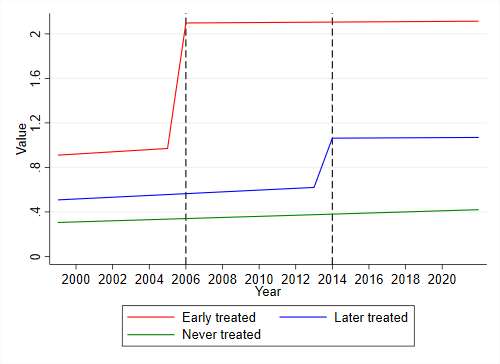
\includegraphics[scale=0.55]{figures/sim_data_f1.png}	
	\end{figure}
	%\begin{minipage}{0.9\linewidth}
	%\fontsize{8}{8pt}\selectfont
	%\emph{Source:} Baker, A. C., Larcker, D. F., and Wang, C. C. (2022)
	%\end{minipage}
\end{frame}



\begin{frame}{Staggered DID design: Conventional Setup}{}
	\begin{itemize}
		\item We obtain DID estimate using the following two-way fixed effect (TWFE) form:
		\vspace{0.2cm}
		\begin{equation*}
			Y_{it} = \alpha_{i} + \lambda_{t}+ \delta^{DD} Treat_{i} \times Post_{t} + \epsilon_{it}.
		\end{equation*}

	\begin{itemize}
	\item $\alpha_{i}$ are unit fixed effects
	\vspace{0.2cm}
		\begin{itemize}
	\item Effects for $Treat_{i}$ is subsumed by the unit fixed effects
\end{itemize}	
	\vspace{0.2cm}
	\item $\lambda_{t}$ are time period fixed effects
	\vspace{0.2cm}
	\begin{itemize}
		\item Effects for $Post_{t}$ is subsumed by the time fixed effects
	\end{itemize}	
	\vspace{0.2cm}
	%\item $\varepsilon_{st}$ is a transitory shock/idiosyncratic error
	%\vspace{0.2cm}
	\item $Treat_{i} \times Post_{t}$ is an indicator for a treated unit in post-treatment periods 
	\vspace{0.2cm}
	
	
	%\item if $E[\varepsilon|D,T]=0$
\end{itemize}	
	
		
		
	\end{itemize}
\end{frame}




\begin{frame}{Staggered DID design: Conventional Setup}{}
	\begin{itemize}
		\item This TWFE regression model can extend to dynamic treatment effect estimation
				\vspace{0.2cm}
			\begin{itemize}		
		\item By separately including indicators for the number of periods before or after the treatment
				\end{itemize}
						\vspace{0.2cm}	
		\begin{equation*}
			Y_{it} = \alpha_{i} + \lambda_{t}+ \sum_{\substack{k\neq-1}}\delta_{k} Treat_{i} \times \mathbf{I}[t-E_{i}=k] + \epsilon_{it}.
		\end{equation*}
		
		\begin{itemize}
			\item  $E_{i}$ represents the timing when treatment happens.
		\vspace{0.2cm}
		\item $\mathbf{I}[t-E_{i}=k]$ is an indicator for being $k$ years from the treatment event
		\vspace{0.2cm}
		\item $t$ is the calendar year
		\vspace{0.2cm}
		\begin{itemize}			
			\item Treatment occurs in $k=0$ ($t=E_{i}$)
			\vspace{0.2cm}
			\item For example, $\mathbf{I}[t-E_{i}=-1]$ is a dummy variable indicating one year before treatment occurs
			\vspace{0.2cm}
			\item We usually use time $k=-1$ as baseline year
			
		\end{itemize}
			
			
			%\item if $E[\varepsilon|D,T]=0$
		\end{itemize}	
		
		
		
	\end{itemize}
\end{frame}






\title[]  
{Conventional TWFE \\ STATA Example}

\author 
{}

\institute{}


\date
{}

\begin{frame}{}
	\titlepage
\end{frame}





\begin{frame}{Data and Program}{}
	\begin{itemize}
		\item See Stag\_DID.do
		\vspace{0.2cm}
		\item Use fert\_rate\_synth.csv
		
		
	\end{itemize}
\end{frame}





\begin{frame}[fragile]{Overview Dataset}	
	\begin{itemize}
		
		
		\item This project examines the effect of paid-parental leave on fertility
		\begin{itemize}
			\item Rhode Island and New York implements paid-parental leave in 2015 and 2018, respectively
			\vspace{0.2cm}		
		\end{itemize}
		
		\item Use staggered DID design to evaluate its impact		
		\vspace{0.2cm}		
		\item The dataset contains state-level fertility rate and other demographic variables from 2007-2021
		\vspace{0.2cm}
		
		
		\begin{itemize}	
			\vspace{0.2cm}	
			\item \textbf{fert:} Fertility rate, which is the outcome variable
			\vspace{0.2cm}
			\item \textbf{year:} This is the year and is the time variable
			\vspace{0.2cm}
			\item \textbf{state:} This is an id number for each state and provides the individual identifier in this panel data context
		\end{itemize}
		
	\end{itemize}
	
	
	
	
\end{frame}



\begin{frame}[fragile]{Step 1: Define Treatment Group and Treatment Timing}{}
\begin{lstlisting}
gen treated_post = 1 if (year>=2018 &  ipums==36) | (year>=2015 &  ipums==44) // New york (36) and Rhode Island (44)

replace treated_post = 0 if treated_post==.
\end{lstlisting}	
	
	
\begin{itemize}
	\vspace{0.2cm}
	\item Create a binary indicator for treatment group and their post-treatment periods ($Treat_{i} \times Post_{t}$)
	\vspace{0.2cm}
	\begin{itemize}
		\item New york (36) and Rhode Island (44) start treatment in 2018 and 2015, respectively
	\end{itemize}
\end{itemize}
	
	
	
	
\end{frame}



\begin{frame}[fragile]{Step 2: TWFE Estimation}{}
\begin{lstlisting}
reg fert treated_post i.year i.state_id, cl(state_id)
reghdfe fert treated_post, absorb(year state_id) vce(cluster state_id)
\end{lstlisting}	
	
	
	\begin{itemize}
		
		\item \textbf{reg}: a TWFE regression model, controlling for year and state fixed effects
		\vspace{0.2cm}
		\item \textbf{reghdfe}: an advanced version of the first, absorbing multiple fixed effects more efficiently
		\vspace{0.2cm}
		\begin{itemize}
			\item Both are clustering standard errors at the state level
		\end{itemize}
	\end{itemize}
	
	
	
	
\end{frame}



\begin{frame}[fragile]{Step 3: Create Variables for Dynamic TWFE Estimation}{}
\begin{lstlisting}
set seed 123456

gen treat_year = .

levelsof ipums, local(levels)

foreach i of local levels {

local randyear = cond(runiform() < 0.5, 2015, 2018)
replace treat_year = `randyear' if ipums == `i'
}

replace treat_year = 2018 if ipums == 36
replace treat_year = 2015 if ipums == 44
\end{lstlisting}	
	
	
 \begin{itemize}
	\item Specify the treatment years to treated states
\vspace{0.2cm}
		\item Randomly assign "treatment years" to different states, with specific assignments for untreated states.
		\vspace{0.2cm}
\end{itemize}
	
	
	
	
\end{frame}




\begin{frame}[fragile]{Step 3: Create Variables for Dynamic TWFE Estimation}{}
\begin{lstlisting}
gen event_year= year - treat_year

forvalue i =8(-1)1 {
gen pre_event_`i'= (event_year == -`i')
}

forvalue i =0(1)3 {
gen post_dd_`i'= (event_year == `i')*treated
}
\end{lstlisting}	
	
	
	\begin{itemize}
		\item Create interaction between treatment group dummy and event time dummies $Treat_{i} \times \mathbf{I}[t-E_{i}=k]$
	
	\end{itemize}
	
	
	
	
\end{frame}



\begin{frame}[fragile]{Step 4: Dynamic TWFE Estimation}{}
\begin{lstlisting}
reghdfe fert treated pre_dd_8-pre_dd_2 post_dd_0 -post_dd_3, absorb(year state_id) vce(cluster state_id)
\end{lstlisting}	
	
	
	\begin{itemize}
		\item Implement dynamic TWFE estimation
		
	\end{itemize}
	
	
	
	
\end{frame}



\title[]  
{Conventional TWFE  \\  Problems and Solutions}


\author 
{}

%\institute{Institute of Economics, Academia Sinica  \\ Econ, NTU}
%\institute{Institute of Economics, Academia Sinica  \\ IMES/IDAS, NCCU}
\institute{}

%\author 
%{楊子霆 \\ 中研院經濟所}

%\institute 
%{中正大學國際經濟專題研討}




\date
{}


\begin{frame}{}
	\titlepage
\end{frame}

\begin{frame}{Staggered DID design: Problems}{}
	\begin{itemize}
	
					\vspace{0.2cm}
		\item Rrecent work in econometric theory indicates that the main coefficient of interest $\delta^{DD}$ is
		not easily interpretable
							\vspace{0.2cm}
		\item Numerous studies have now shown that this coefficient is in fact a weighted average of
		many different treatment effects
		\vspace{0.2cm}
		\begin{itemize}
			\item Can yield estimates with the opposite sign compared to the
			true ATE or ATT
		\end{itemize}
		
	\end{itemize}
\end{frame}





\begin{frame}{Staggered DID design: Problems}{}
	\begin{itemize}
		\item Goodman-Bacon (2019) decomposes $\delta^{DD}$  in a stylized setting where there are  three groups:
		\vspace{0.2cm}
		\begin{itemize}
			\item[1] a never-treated group (denoted U)
					\vspace{0.2cm}
			\item[2] an early-treatment group (denoted E) that is
			treated at year 2006 ($t^{*}_{E}$)
			\vspace{0.2cm}
			\item[3] a late-treatment group (denoted L) that is treated at year 2014 ($t^{*}_{L}$)
		\end{itemize}
		
		
	\end{itemize}
\end{frame}

\begin{frame}{Staggered DID design: Problems}{Examples}
	\begin{figure}[H]
		\centering
		%
\includegraphics[scale=0.7]{figures/f4.png}	
				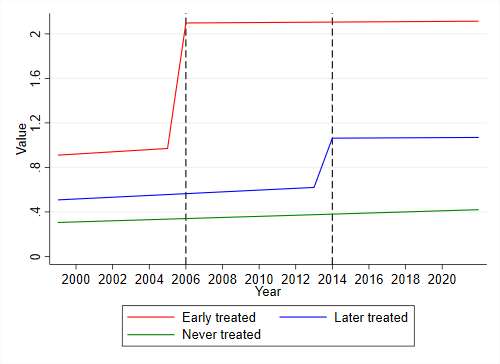
\includegraphics[scale=0.55]{figures/sim_data_f1.png}	
	\end{figure}
	%\begin{minipage}{0.9\linewidth}
	%\fontsize{8}{8pt}\selectfont
	%\emph{Source:} Baker, A. C., Larcker, D. F., and Wang, C. C. (2022)
%\end{minipage}
\end{frame}



\begin{frame}{Staggered DID design: Problems}{}
\begin{itemize}

	\item There are three sub-periods in this set up:
	\vspace{0.2cm}
	\begin{itemize}
		\item The pre-treatment period for group $E$:  $T1 = [2000, 2005]$
		\vspace{0.2cm}
		\item The middle period when group $E$ is treated but group $L$ is not: $T2=[2006, 2013]$
		\vspace{0.2cm}
		\item The post-treatment period for group $L$: $T3=[2014, 2022]$		
	\end{itemize}
	
\end{itemize}
\end{frame}


\begin{frame}{Staggered DID design: Problems}{Examples}
	\begin{itemize}
		\item  Goodman-Bacon (2019) shows that in this three-group case, $\delta^{DD}$ is a weighted average of four possible 2x2 DID comparisons
		\vspace{0.2cm}
		\begin{itemize}
			\item[1] an early-treatment group v.s. a never-treated group 
			\vspace{0.2cm}
			\item[2] a late-treatment group v.s. a never-treated group 
			\vspace{0.2cm}
			\item[3] an early-treatment group v.s. a late-treatment group 
							\vspace{0.2cm}
					\begin{itemize}
			\item Before year 2014 ($t^{*}_{L}$) 
					\end{itemize}
				\vspace{0.2cm}
			\item[4] a late-treatment group v.s. an early-treatment group 
				\vspace{0.2cm}
			\begin{itemize}
			\item After year 2006 ($t^{*}_{E}$) 
					\end{itemize}
		\end{itemize}
	
		
	\end{itemize}
\end{frame}






\begin{frame}{An early-treatment group v.s. A never-treated group }{}
	\begin{itemize}
		\item  In this case,
		the TWFE estimate of $\delta^{DD}$ reduces to the standard 2x2 DID estimate
		\vspace{0.2cm}
	\begin{equation*}
		\hat{\delta}_{EU}=\left( \Bar{y}^{T2+T3}_{E} - \Bar{y}^{T1}_{E}\right) - \left( \Bar{y}^{T2+T3}_{U} - \Bar{y}^{T1}_{U}\right)
	\end{equation*}
		
		
	\end{itemize}
\end{frame}



\begin{frame}{An early-treatment group v.s. A never-treated group }{}
	\begin{figure}[H]
		\centering
		%\includegraphics[scale=1.0]{figures/f4a.png}	
		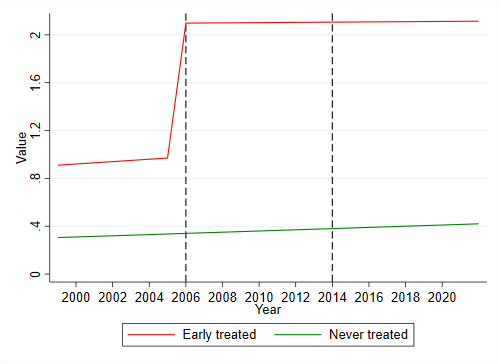
\includegraphics[scale=0.55]{figures/sim_data_f2.png}		
	\end{figure}
	%\begin{minipage}{0.9\linewidth}
%\fontsize{8}{8pt}\selectfont
%\emph{Source:} Baker, A. C., Larcker, D. F., and Wang, C. C. (2022)
%\end{minipage}
\end{frame}


\begin{frame}{A late-treatment group v.s. A never-treated group}{}
	\begin{itemize}
		\item  In this case,
		the TWFE estimate of $\delta^{DD}$ reduces to the standard 2x2 DID estimate
		\vspace{0.2cm}
	\begin{equation*}
		\hat{\delta}_{LU}=\left( \Bar{y}^{T3}_{L} - \Bar{y}^{T1+T2}_{L}\right) - \left( \Bar{y}^{T3}_{U} - \Bar{y}^{T1+T2}_{U}\right).
	\end{equation*}
		
		
	\end{itemize}
\end{frame}



\begin{frame}{A late-treatment group v.s. A never-treated group}{}
	\begin{figure}[H]
		\centering
		%\includegraphics[scale=1.0]{figures/f4b.png}
				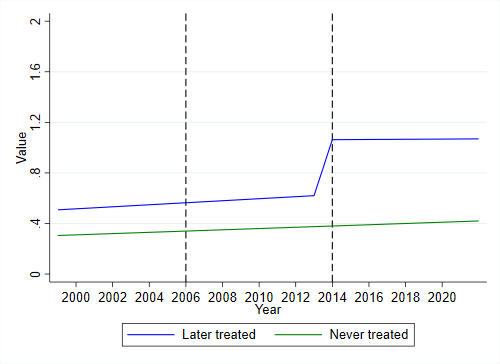
\includegraphics[scale=0.55]{figures/sim_data_f3.png}			
	\end{figure}
	%\begin{minipage}{0.9\linewidth}
%\fontsize{8}{8pt}\selectfont
%\emph{Source:} Baker, A. C., Larcker, D. F., and Wang, C. C. (2022)
%\end{minipage}
\end{frame}


\begin{frame}{An early-treatment group v.s. A late-treatment group}{}
	\begin{itemize}
		\item  In the following
		cases, the TWFE estimate of $\delta^{DD}$ is identified from the difference in the \textbf{timing} of the treatments between \textbf{treatment groups}
		
		\item We compare the
		early-treated group to later-treated group in a window  (before year 2014 $t^{*}_{L}$) 
		\vspace{0.2cm}
			\begin{itemize}
			\item Treatment group: early-treated units
			\vspace{0.2cm}
				\begin{itemize}
			\item Treatment status varies in the early-treated units		
				\end{itemize}
						\vspace{0.2cm}			
			\item Control group: Later-treated units
		\vspace{0.2cm}
		\begin{itemize}
			\item Later-treated units do not receive treatment	
		\end{itemize}			
		\end{itemize}	
				\vspace{0.2cm}	
	\begin{equation*}
		\hat{\delta}_{EL}=\left( \Bar{y}^{T2}_{E} - \Bar{y}^{T1}_{E}\right) - \left( \Bar{y}^{T2}_{L} - \Bar{y}^{T1}_{L}\right).
	\end{equation*}
		
		
	\end{itemize}
\end{frame}


\begin{frame}{An early-treatment group v.s. A late-treatment group}{}
	\begin{figure}[H]
		\centering
		%\includegraphics[scale=1.0]{figures/f4c.png}
			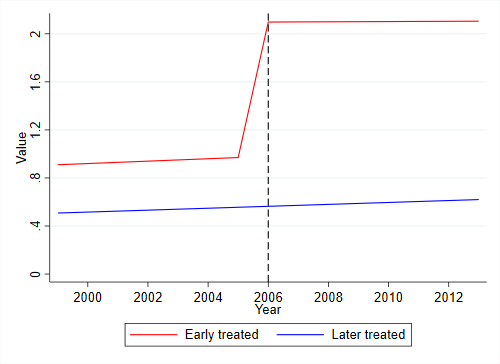
\includegraphics[scale=0.55]{figures/sim_data_f4.png}				
	\end{figure}
	%\begin{minipage}{0.9\linewidth}
%\fontsize{8}{8pt}\selectfont
%\emph{Source:} Baker, A. C., Larcker, D. F., and Wang, C. C. (2022)
%\end{minipage}
\end{frame}



\begin{frame}{A late-treatment group v.s. An early-treatment group}{}
	\begin{itemize}
		
		\item We compare the early-treated group to
		later-treated group in a window (after year 2006 $t^{*}_{E}$)
		\vspace{0.2cm}
	\begin{itemize}
		\item Treatment group: Later-treated units
	\vspace{0.2cm}
	\begin{itemize}
		\item Treatment status varies in the later-treated units
	\end{itemize}
	\vspace{0.2cm}
		\item Control group: Early-treated units
		\vspace{0.2cm}
	\begin{itemize}
		\item Early-treated units do not receive treatment	
	\end{itemize}	
			\vspace{0.2cm}
	\end{itemize}	
		
		
		\begin{equation*}
			\hat{\delta}_{LE}=\left( \Bar{y}^{T3}_{L} - \Bar{y}^{T2}_{L}\right) - \left( \Bar{y}^{T3}_{E} - \Bar{y}^{T2}_{E}\right).
		\end{equation*}

	\item In such a setting, the potential for bias	in $\delta^{DD}$ could be large
						\vspace{0.2cm}
		\begin{itemize}
	\item If the treatment effect is increasing over time, the change in outcomes of the early-treated group could be substantial
		\end{itemize}
	
	
	%the large changes in the outcome for earlier treated firms, which are used as effective comparison units, are subtracted from the relatively smaller changes in the outcome for later treated firms, which are the effective treatment firms.
	
	
	%The outcomes of the early-treated group could 		
	%\item When the later-treated group receive treatment, the changes in the outcomes of later-treated are relatively small compared to the contemporaneous changes in the outcomes of the early-treated group	
		
	\end{itemize}
\end{frame}



\begin{frame}{A late-treatment group v.s. An early-treatment group}{}
	\begin{figure}[H]
		\centering
		%\includegraphics[scale=1.0]{figures/f4d.png}
			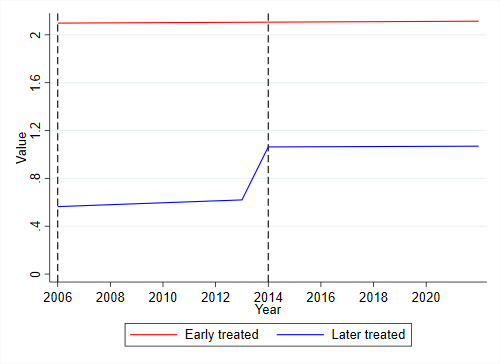
\includegraphics[scale=0.55]{figures/sim_data_f5.png}				
	\end{figure}
	%\begin{minipage}{0.9\linewidth}
%\fontsize{8}{8pt}\selectfont
%\emph{Source:} Baker, A. C., Larcker, D. F., and Wang, C. C. (2022)
%\end{minipage}
\end{frame}



\begin{frame}{Summary of Goodman-Bacon (2019) Derivation}{}
	\begin{itemize}
		\item  Two main insights that follow from the Goodman-Bacon (2019) derivation:
		\vspace{0.2cm}
		\begin{itemize}
			\item[1] The TWFE estimate $\delta^{DD}$ in a staggered DID design is the weighted average of the several 2x2 DID estimate
			\vspace{0.2cm}
			\item[2] Among these 2x2 DID estimate, some of control groups are also treated, which results in bias 
			\vspace{0.2cm}
%			\item[3] The contribution of each 2x2 DID to the TWFE estimate $\delta^{DD}$ is sample dependent
%			\vspace{0.2cm}
%			\begin{itemize}
%				\item The treatment groups receive treatment closer to the middle of the panel receive greater weight
%				\vspace{0.2cm}
%				\item Because the variance of the treatment indicator is maximized when groups have roughly equal treated and untreated periods
%				\vspace{0.2cm}
%				\item Intuitively, TWFE model gives more weight to groups that provide the most balanced "before-after" comparison, which happens to be those treated in the middle of the study period
%			\end{itemize}
		\end{itemize}
		
		
	\end{itemize}
\end{frame}



%
%\begin{frame}{Summary of Goodman-Bacon (2019) Derivation}{}
%\begin{itemize}
%	\item  Three main insights that follow from the Goodman-Bacon (2019) derivation:
%	\vspace{0.2cm}
%	\begin{itemize}
%		\item[1] The TWFE estimate $\delta^{DD}$ in a staggered DID design is the weighted average of the several 2x2 DID estimate
%		\vspace{0.2cm}
%		\item[2] Among these 2x2 DID estimate, some of control groups are also treated, which results in bias 
%		\vspace{0.2cm}
%		\item[3] The contribution of each 2x2 DID to the TWFE estimate $\delta^{DD}$ is sample dependent
%		\vspace{0.2cm}
%			\begin{itemize}
%		\item The treatment groups receive treatment closer to the middle of the panel receive greater weight
%				%\vspace{0.2cm}
%		%\item Because the variance is the treatment indicator variable is larger.
%			\end{itemize}
%	\end{itemize}
%	
%	
%\end{itemize}
%\end{frame}




\begin{frame}{Staggered DID design: Solutions}{}
\begin{itemize}
	\item  There are several alternative DID estimators that deal with this issue
	\vspace{0.2cm}
	\begin{itemize}
		\item Has not yet settled on an established standard
		\vspace{0.2cm}
		\item Implement at least one such method to test the robustness of your DID estimate
		\vspace{0.2cm}
	
		\end{itemize}
	
	\item \textbf{Intuition:} Avoids "problematic comparisons" in which already treated units serve as control group
			\vspace{0.2cm}
	\item Use clean controls: 
			\vspace{0.2cm}
				\begin{itemize}
	\item Never treated units 
			\vspace{0.2cm}
	\item Not-yet-treated units
		\end{itemize}
	%units that are treated far enough in the future to provide a clean post-period.
	
	\end{itemize}
	
	
\end{frame}



\begin{frame}{Staggered DID design: Solutions}{Callaway and Sant'Anna Estimator}
	\begin{itemize}
		\item  Callaway and Sant'Anna (2020) proposes a two-step estimation strategy with a bootstrap procedure
		\vspace{0.2cm}
		\begin{itemize}
			\item \textbf{Step 1:} Compute all possible "clean" \textbf{group-time average treatment effects $ATT (g,t)$}
			\vspace{0.2cm}
			\item \textbf{Step 2:} Aggregating these group-time average treatment effects to obtain single number $ATT$
			\vspace{0.2cm}
					\begin{itemize}
			\item Utilize bootstrap procedure to calculate standard error of Callaway and Sant'Anna's DID estimate
					\end{itemize}
			
		\end{itemize}
		
		
		
	\end{itemize}
	
	
\end{frame}


\begin{frame}{Callaway and Sant'Anna Estimator}{Notations}
	\begin{itemize}
	
			\item $Y_{it}(0)$: unit $i$'s potential outcome in period $t$ if they do not participate in the treatment
			\vspace{0.2cm}
			\item $Y_{it}(g)$:	unit $i$'s potential outcome in time period $t$
			if they become treated in period $g$
			\vspace{0.2cm}
				\item $G_{i}$: the time period when unit $i$ becomes treated 
		\vspace{0.2cm}				
		\item $C_{i}$: an indicator variable for whether unit i
		is in a never-treated group
		\vspace{0.2cm}
		\item 	$D_{it}$: an indicator variable for whether unit $i$
		has been treated by time $t$
			
		\end{itemize}
		


\end{frame}





\begin{frame}{Callaway and Sant'Anna Estimator}{Notations}
	\begin{itemize}
	

		\item 	$Y_{it}$: unit $i$'s observed outcome in time period  $t$	 		
			\vspace{0.2cm}
		\begin{itemize}	
		\item For units in early or later treatment groups:
			
		\begin{equation*}
			Y_{it} = 1\{G_i>t\} \times Y_{it}(0)+1\{G_i \leq t\} \times Y_{it}(G_{i})
		\end{equation*}
						\end{itemize}
		
			\vspace{0.2cm}
		\begin{itemize}	
			\item For units in the never-treated group:
			
			\begin{equation*}
				Y_{it} = Y_{it}(0)
			\end{equation*}
		\end{itemize}
		
			
		\end{itemize}

	
\end{frame}





\begin{frame}{Callaway and Sant'Anna DID Estimator}{Step 1: Group-Time Average Treatment Effects}
	\begin{itemize}
		%\item  Generalize ATT from the two periods and two groups case to the multiple periods case
		%\vspace{0.2cm}
		\item Group-time average treatment effects:
		
		\begin{equation*}
	    ATT (g,t) \equiv \mathbb{E}\left[Y_{it}(g)-Y_{it}(0) | G_{i}=g \right].
		\end{equation*}
		
		
		\item Groups are basically cohorts of units treated at the same time
						\vspace{0.2cm}
		\item This is the average effect of participating in the treatment for units in group $g$ at time period $t$
				\vspace{0.2cm}
		%\item Examples:
			\begin{itemize}
		\item $ATT(g=2,t=2)$: average effect of participating in the treatment for the group of units that become treated in time period 2, in time period 2
						\vspace{0.2cm}
		\item $ATT(g=2,t=3)$: average effect of participating in the treatment for the group of units that become treated in time period 2, in time period 3
		
		
			\end{itemize}
		
		
	\end{itemize}
	
	
\end{frame}




\begin{frame}{Callaway and Sant'Anna DID Estimator}{Assumptions and Identification}
	\begin{itemize}
		
		\item  In the multiple periods case, we will have many group-time average treatment effects $ATT (g,t)$
				\vspace{0.2cm}
			\begin{itemize}
		\item Identify each $ATT (g,t)$ using "clean" control groups
						\vspace{0.2cm}
		\begin{itemize}
			\item Never treated units 
			\vspace{0.2cm}
			\item Not-yet-treated units
		\end{itemize}
		
			\end{itemize}
		
	
		
		
	\end{itemize}
	
	
\end{frame}




\begin{frame}{Callaway and Sant'Anna DID Estimator}{Assumptions and Identification}
	\begin{itemize}
		
		\item  Parallel Trends Assumption based on \textbf{never-treated units}:
		\vspace{0.2cm}
			\begin{itemize}
		\item For all $g=2,...,\mathcal{T}$ and $s,t=2,...,\mathcal{T}$ with $t \ge g$
			\end{itemize}
				\vspace{0.2cm}
		
		\begin{equation*}
			\mathbb{E}\left[Y_{t}(0)-Y_{t-1}(0) | G=g \right] = 	\mathbb{E}\left[Y_{t}(0)-Y_{t-1}(0) | C=1 \right].
		\end{equation*}
									\vspace{0.2cm}
		
		\item  Identification of group-time average treatment effects:
		
		\begin{equation*}
			ATT (g,t) \equiv	\mathbb{E}\left[Y_{t}-Y_{g-1} | G=g \right] - 	\mathbb{E}\left[Y_{t}-Y_{g-1} |C=1 \right].
		\end{equation*}
		
		
	\end{itemize}
	
	
\end{frame}



\begin{frame}{An early-treatment group v.s. A never-treated group }{}
\begin{figure}[H]
	\centering
	%\includegraphics[scale=1.0]{figures/f4a.png}	
	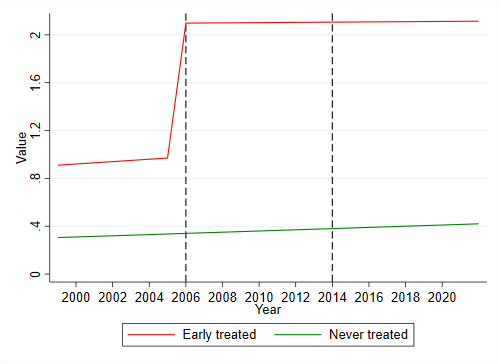
\includegraphics[scale=0.55]{figures/sim_data_f2.png}		
\end{figure}
%\begin{minipage}{0.9\linewidth}
%\fontsize{8}{8pt}\selectfont
%\emph{Source:} Baker, A. C., Larcker, D. F., and Wang, C. C. (2022)
%\end{minipage}
\end{frame}





\begin{frame}{A late-treatment group v.s. A never-treated group}{}
\begin{figure}[H]
	\centering
	%\includegraphics[scale=1.0]{figures/f4b.png}
	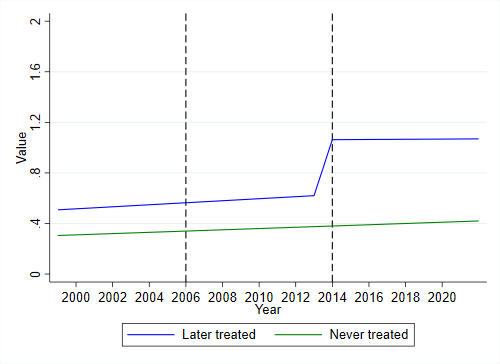
\includegraphics[scale=0.55]{figures/sim_data_f3.png}			
\end{figure}
%\begin{minipage}{0.9\linewidth}
%\fontsize{8}{8pt}\selectfont
%\emph{Source:} Baker, A. C., Larcker, D. F., and Wang, C. C. (2022)
%\end{minipage}
\end{frame}


\begin{frame}{Callaway and Sant'Anna DID Estimator}{Assumptions and Identification}
	\begin{itemize}
	
		
		\item  Parallel Trends Assumption based on \textbf{not-yet treated units}:
		\vspace{0.2cm}
					\begin{itemize}
				\item For all $g=2,...,\mathcal{T}$ and $s,t=2,...,\mathcal{T}$ with $t \ge g$ and $s \ge t$
							\end{itemize}
								\vspace{0.2cm}
		\begin{equation*}
			\mathbb{E}\left[Y_{t}(0)-Y_{t-1}(0) | G=g \right] = 	\mathbb{E}\left[Y_{t}(0)-Y_{t-1}(0) | D_{s}=0, G \neq g \right].
		\end{equation*}
									\vspace{0.2cm}
			\item  Identification of group-time average treatment effects:
		
		\begin{equation*}
			ATT (g,t) \equiv	\mathbb{E}\left[Y_{t}-Y_{g-1} | G=g \right] - 	\mathbb{E}\left[Y_{t}-Y_{g-1} |D_{s}=0, G \neq g \right].
		\end{equation*}
		
		
	\end{itemize}
	
	
\end{frame}



\begin{frame}{An early-treatment group v.s. A late-treatment group}{}
	\begin{figure}[H]
		\centering
		%\includegraphics[scale=1.0]{figures/f4c.png}
		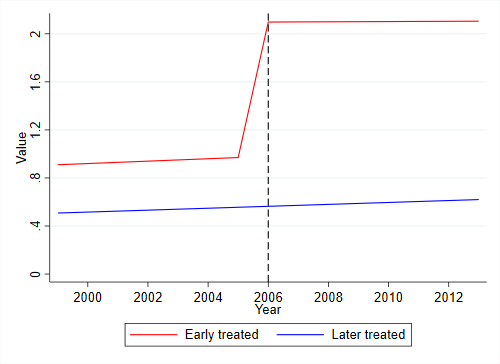
\includegraphics[scale=0.55]{figures/sim_data_f4.png}				
	\end{figure}
	%\begin{minipage}{0.9\linewidth}
	%\fontsize{8}{8pt}\selectfont
	%\emph{Source:} Baker, A. C., Larcker, D. F., and Wang, C. C. (2022)
	%\end{minipage}
\end{frame}



\begin{frame}{Callaway and Sant'Anna DID Estimator}{Step 2: Aggregating Group-Time Average Treatment Effects}
	\begin{itemize}
		
		\item It can be hard to summarize group-time average treatment effects $ATT (g,t)$ to a single number
					\vspace{0.2cm}
		\item Callaway and Sant'Anna (2021) propose a number of ways to aggregate group-time average treatment effects
							\vspace{0.2cm}
		
		\end{itemize}
	
\end{frame}



\begin{frame}{Callaway and Sant'Anna DID Estimator}{Average Treatment Effects for a Specific Treated Cohort}
	\begin{itemize}
		
	
		
		\item[1]  The average effect of participating in the treatment, separately for each treated group $g$
		\vspace{0.2cm}
		\begin{equation*}
			\theta_S(g) = \frac{1}{\mathcal{T} - g + 1} \sum_{t=2}^{\mathcal{T}} \mathbf{1}\{g \leq t\} \times  ATT(g,t).
		\end{equation*}
	\end{itemize}
	
\end{frame}




\begin{frame}{Callaway and Sant'Anna DID Estimator}{Average Treatment Effects on Treated}
	\begin{itemize}
		
		\item[2] It is fairly straightforward to further aggregate $\theta_S(g)$ to get an easy-to-interpret average treatment effects on treated
		
		\begin{equation*}
			\theta^O_S := \sum_{g=2}^{\mathcal{T}} \theta_S(g) \times Pr(G=g).
		\end{equation*}
		
		\item $Pr(G=g)$ is the probability (or proportion) of units belonging to treatment group $g$
				\vspace{0.2cm}
%		\begin{itemize}
%			\item $G=g$ denotes the group that first receives treatment in period $g$
%					\vspace{0.2cm}
%			\item $Pr(G=g)$ serves as a weight that reflects the relative size of each treatment group
%		\end{itemize}
%		\vspace{0.2cm}
		
		\item $\theta^O_S$ is the overall effect of participating in the treatment across all groups that have ever participated in the treatment
		\vspace{0.2cm}
	    \item This is close to being a multi-period analogue of the ATT
	in the two period case
	
		
		
	\end{itemize}
\end{frame}



%
%\begin{frame}{Callaway and Sant'Anna DID Estimator}{Average Treatment Effects on Treated}
%	\begin{itemize}
%		
%
%		\item[2] It is fairly straightforward to further aggregate $\theta_S(g)$ to get an easy-to-interpret average treatment effects on treated
%		
%		\begin{equation*}
%			\theta^O_S := \sum_{g=2}^{\mathcal{T}} \theta_S(g) \times P(G=g).
%		\end{equation*}
%		
%	\item $\theta^O_S$ is the overall effect of participating in the treatment across all groups that have ever participated in the treatment
%		\vspace{0.2cm}
%    \item This is close to being a multi-period analogue of the ATT
%    in the two period case
%    
%  
%		\end{itemize}
%\end{frame}




\begin{frame}{Callaway and Sant'Anna DID Estimator}{Dynamic Average Treatment Effects on Treated}
	\begin{itemize}
		\item[3] We can also get dynamic ATT by calculating ATT at event time $e$:
	
		\begin{equation*}
			\theta_D(e) := \sum_{g=2}^{\mathcal{T}} \mathbf{1} \{ g + e \leq \mathcal{T} \} \times ATT(g,g+e) \times Pr(G=g | G+e \leq \mathcal{T}).
		\end{equation*}
		%\item Where:
		\begin{itemize}
			\item $e$ is the number of periods relative to initial treatment (event time)
					\vspace{0.2cm}
			\item $\mathbf{1} \{ g + e \leq \mathcal{T} \}$ is an indicator ensuring we only include groups observable at event time $e$
					\vspace{0.2cm}
			\item $Pr(G=g | G+e \leq \mathcal{T})$ is the conditional probability of being in group $g$ among all groups that can be observed at event time $e$
		\end{itemize}
		\vspace{0.2cm}
		\item Simple Example ($e=1$ year after treatment):
		\vspace{0.2cm}
		\begin{itemize}
			\item Group treated in 2006: Look at 2007 effect
			\vspace{0.2cm}
			\item Group treated in 2014: Look at 2015 effect
			\vspace{0.2cm}
			\item Average these effects across groups, weighted by their relative sizes
		\end{itemize}
		
	\end{itemize}
\end{frame}



\begin{frame}{Callaway and Sant'Anna DID Estimator}{Dynamic Average Treatment Effects on Treated}
	\begin{itemize}
		\item[3] We can also get dynamic ATT
		\vspace{0.2cm}
		\item Formula for ATT at event time $e$:
		\begin{equation*}
		\theta_D(e) := \sum_{g=2}^{\mathcal{T}} \mathbf{1} \{ g + e \leq \mathcal{T} \} \times ATT(g,g+e) \times P(G=g | G+e \leq \mathcal{T}).
	\end{equation*}
		\item Simple Example ($e=2$ years after treatment):
		\vspace{0.2cm}
		\begin{itemize}
			\item Group treated in 2006: Look at 2007 effect
			\vspace{0.2cm}
			\item Group treated in 2014: Look at 2015 effect
			\vspace{0.2cm}
			\item Average these effects across groups
		\end{itemize}
		
	\end{itemize}
\end{frame}






%
%
%
%\title[]  
%{Staggered DID Design: R Example}
%
%\author 
%{}
%
%\institute{}
%
%
%\date
%{}
%
%\begin{frame}{}
%	\titlepage
%\end{frame}
%
%
%\begin{frame}[fragile]{R Example}{Install package \textbf{did}}
%\begin{lstlisting}
%Install.package("did")
%library(did) 
%\end{lstlisting}	
%	\begin{itemize}
%		\vspace{0.2cm}
%		\item The \textbf{did} package contains tools for computing average treatment effect parameters in a Difference-in-Differences setup allowing for
%		\vspace{0.2cm}		
%		\begin{itemize}	
%			\vspace{0.2cm}	
%			\item More than two time periods
%			\vspace{0.2cm}
%			\item Variation in treatment timing (i.e., units can become treated at different points in time)
%			\vspace{0.2cm}
%			\item Treatment effect heterogeneity
%			\vspace{0.2cm}
%			\item The parallel trends assumption holds only after conditioning on covariates
%		\end{itemize}
%		
%	\end{itemize}
%	
%	
%	
%	
%\end{frame}
%
%
%
%
%
%
%
%\begin{frame}[fragile]{R Example}{Overview Dataset}
%\begin{lstlisting}
%mpdata <- read.csv(paste0(rdata,"mpdata.csv"))
%
%head(mpdta)
%\end{lstlisting}	
%	
%	
%	\begin{itemize}
%		\vspace{0.2cm}
%		\item The dataset contains 500 observations of county-level teen employment rates from 2003-2007
%				\vspace{0.2cm}
%		\item Some states are first treated in 2004, some in 2006, and some in 2007		
%				\vspace{0.2cm}		
%	
%		
%	\end{itemize}
%	
%\end{frame}
%
%
%
%
%
%\begin{frame}[fragile]{R Example}{Overview Dataset}
%\begin{lstlisting}
%mpdata <- read.csv(paste0(rdata,"mpdata.csv"))
%
%head(mpdta)
%\end{lstlisting}	
%	
%	
%	\begin{itemize}
%		\item Outcome variable:	
%		\vspace{0.2cm}		
%		\begin{itemize}	
%			
%			\item \textbf{lemp:} This is the log of county-level teen employment
%			\vspace{0.2cm}
%		\end{itemize}
%		\item Group variables:
%		\vspace{0.2cm}	
%		\begin{itemize}			
%			\item \textbf{first.treat:} This is the period when a state first increases its minimum wage. 
%			\vspace{0.2cm}	
%			\item It can be 2004, 2006, or 2007. 
%			\vspace{0.2cm}					
%			\item It is the variable that defines group in this application
%			\vspace{0.2cm}
%		\end{itemize}	
%					
%			\item \textbf{year:} This is the year and is the time variable
%			\vspace{0.2cm}
%	
%			\item \textbf{countyreal:} This is an id number for each county and provides the individual identifier in this panel data context
%
%		
%	\end{itemize}
%	
%	
%	
%	
%	
%\end{frame}
%
%
%
%
%\begin{frame}[fragile]{R Example}{Step 1: Estimate group-time average treatment effects}
%\begin{lstlisting}
%out <- att_gt(yname = "lemp",
%gname = "first.treat",
%idname = "countyreal",
%tname = "year",
%xformla = ~1,
%data = mpdta,
%est_method = "reg"
%)
%\end{lstlisting}	
%	
%	
%	\begin{itemize}
%		\vspace{0.2cm}
%		\item \textbf{att\_gt}: Estimate group-time average treatment effects without covariates
%				\vspace{0.2cm}
%			\begin{itemize}
%	\item \textbf{xformla = \textasciitilde 1}: Not include covariates
%			\end{itemize}
%	\end{itemize}
%	
%	
%	
%	
%\end{frame}
%
%
%\begin{frame}[fragile]{R Example}{Step 1: Estimate group-time average treatment effects}
%\begin{lstlisting}
%out.X <- att_gt(yname = "lemp",
%gname = "first.treat",
%idname = "countyreal",
%tname = "year",
%xformla = ~lpop,
%data = mpdta,
%)
%\end{lstlisting}	
%	
%	
%	\begin{itemize}
%		\vspace{0.2cm}
%		\item \textbf{att\_gt}: Estimate group-time average treatment effects without covariates
%		\vspace{0.2cm}
%		\begin{itemize}
%			\item \textbf{xformla = \textasciitilde lpop}: Include covariates \textbf{lpop}
%		\end{itemize}
%	\end{itemize}
%	
%	
%	
%	
%\end{frame}
%
%
%
%
%\begin{frame}[fragile]{R Example}{Step 1: Estimate group-time average treatment effects}
%\begin{lstlisting}
%summary(out)
%ggdid(out, ylim = c(-.25,.1))
%\end{lstlisting}	
%	\begin{itemize}
%		\vspace{0.2cm}
%	\item \textbf{summary(out)}: Summarize the results in out
%	\vspace{0.2cm}	
%		\item \textbf{ggdid(out)}: Plot the group-time average treatment effects
%		\vspace{0.2cm}	
%		
%	\end{itemize}
%
%\end{frame}
%
%
%
%\begin{frame}[fragile]{R Example}{Step 2: Aggregating Group-Time Average Treatment Effects}
%\begin{lstlisting}
%es <- aggte(out, type = "dynamic")
%summary(es)
%ggdid(es)
%\end{lstlisting}	
%	\begin{itemize}
%		\vspace{0.2cm}
%		\item \textbf{aggte()}: Aggregate the group-time average treatment effects into a small number of parameters
%		\vspace{0.2cm}	
%		\item \textbf{type = "dynamic"}: Type of aggregation is average effects computed at each length of exposure (event study) 
%		\vspace{0.2cm}	
%		\item \textbf{ggdid(es)}: Plot the dynamic average treatment effects
%	\end{itemize}
%	
%\end{frame}
%
%
%
%\begin{frame}[fragile]{R Example}{Step 2: Aggregating Group-Time Average Treatment Effects}
%\begin{lstlisting}
%group_effects <- aggte(out, type = "group")
%summary(group_effects)
%\end{lstlisting}	
%	\begin{itemize}
%		\vspace{0.2cm}
%		\item \textbf{type = "group"}: Type of aggregation is averaging the average effects computed at each length of exposure
%		\vspace{0.2cm}	
%		\item This estimate can represent average Treatment Effect on the Treated (ATT)
%	\end{itemize}
%	
%\end{frame}
%


\title[]  
{Callaway and Sant'Anna DID Estimator \\ STATA Example}


\author 
{}

%\institute{Institute of Economics, Academia Sinica  \\ Econ, NTU}
%\institute{Institute of Economics, Academia Sinica  \\ IMES/IDAS, NCCU}
\institute{}

%\author 
%{楊子霆 \\ 中研院經濟所}

%\institute 
%{中正大學國際經濟專題研討}




\date
{}


\begin{frame}{}
	\titlepage
\end{frame}


\begin{frame}{Data and Program}{}
	\begin{itemize}
		\item See Stag\_DID.do
		\vspace{0.2cm}
		\item Use fert\_rate\_synth.csv
		
		
	\end{itemize}
\end{frame}

\begin{frame}[fragile]{Step 0: Install Packages}
\begin{lstlisting}
ssc install csdid
ssc install drdid
\end{lstlisting}	
	
	
	\begin{itemize}
		\vspace{0.2cm}
		\item \textbf{csdid}: Implement Callaway and Sant'Anna DID estimator
		\vspace{0.2cm}
		\begin{itemize}
			\item \textbf{drdid}: Implement doubly robust estimation used in Callaway and Sant'Anna DID estimator
		\end{itemize}
	\end{itemize}
	
	
	
	
\end{frame}



\begin{frame}[fragile]{Step 1: Estimate group-time average treatment effects}
\begin{lstlisting}
csdid fert, ivar(state_id) time(year) gvar(first_treat)  agg(attgt)

csdid_plot, group(2018)
csdid_plot, group(2015)
\end{lstlisting}	
	
	
	\begin{itemize}
		\vspace{0.2cm}
		\item \textbf{ivar()}: indicating panel variable
		\vspace{0.2cm}
			\item \textbf{time()}: indicating time variable 
			\vspace{0.2cm}
		\item \textbf{gvar()}: indicating period when an unit is first treated
					\vspace{0.2cm}
		\item \textbf{agg(attgt)}: Estimate group-time average treatment effects			
										\vspace{0.2cm}
		\item \textbf{csdid\_plot}: Display the dynamic effect of treatment for each treatment group
	\end{itemize}
	
	
	
	
\end{frame}


\begin{frame}[fragile]{Step 2: Aggregating Group-Time Average Treatment Effects}{Dynamic Average Treatment Effects on Treated}
\begin{lstlisting}
csdid fert, ivar(state_id) time(year) gvar(first_treat) agg(event)

csdid_plot
\end{lstlisting}	
	
	
	\begin{itemize}
		\vspace{0.2cm}
		\item \textbf{agg(event)}: Estimate dynamic treatment effects			
		\vspace{0.2cm}
		\item \textbf{csdid\_plot}: Display the dynamic effect of treatment
	\end{itemize}
	
	
	
	
\end{frame}


\begin{frame}[fragile]{Step 2: Aggregating Group-Time Average Treatment Effects}{Average Treatment Effects on Treated}
\begin{lstlisting}
csdid fert, ivar(state_id) time(year) gvar(first_treat) agg(simple)
\end{lstlisting}	
	
	
	\begin{itemize}
		\vspace{0.2cm}
		\item \textbf{agg(simple)}: Estimate average treatment effect			
	\end{itemize}
	
	
	
	
\end{frame}



\begin{frame}[fragile]{Step 2: Aggregating Group-Time Average Treatment Effects}
\begin{lstlisting}
csdid fert unemploymentrate , ivar(state_id) time(year) gvar(first_treat)
estat all
\end{lstlisting}	
	
	
	\begin{itemize}
		\vspace{0.2cm}
		\item \textbf{estat all}: Display all estimates		
	\end{itemize}
	
	
	
	
\end{frame}




\title[]{Callaway and Sant'Anna DID Estimator \\ R Example}

\author{}

\institute{}

\date{}

	
	\begin{frame}
		\titlepage
	\end{frame}

\begin{frame}{Data and Program}{}
	\begin{itemize}
		\item See Stag\_DID.R
		\vspace{0.2cm}
		\item Use fert\_rate\_synth.csv
		
		
	\end{itemize}
\end{frame}


	
	\begin{frame}[fragile]{Step 0: Setup Environment}
\begin{lstlisting}[language=R]
library(data.table)  # for data manipulation
library(did)         # for DiD estimation
\end{lstlisting}
		
		\begin{itemize}
			\item \textbf{data.table}: Efficient data manipulation.
					\vspace{0.2cm}
			\item \textbf{did}: Implement Callaway and Sant'Anna DID estimator.
		\end{itemize}
		
	\end{frame}
	
\begin{frame}[fragile]{Step 1: Data Preparation}

\begin{lstlisting}[language=R]
# Import the dataset using fread
fert_rate_synth <- fread(file.path(rdata, "fert_rate_synth.csv"), header = TRUE, data.table = TRUE)

# Drop CA, NJ, WA based on their state codes
fert_rate_synth <- fert_rate_synth[!ipums %in% c(6, 34, 53)]
\end{lstlisting}
	\begin{itemize}

		\item \textbf{fread} function is part of the \textit{data.table} package, used for fast and efficient import of data
							\vspace{0.2cm}
		\item \textbf{file.path} ensures that the file path is correctly formed across different operating systems
							\vspace{0.2cm}
		\item Options: \textbf{header} indicates whether the first line of the file contains column names, \textbf{data.table = TRUE} ensures that the output is a data.table object
							\vspace{0.2cm}
		\item \textbf{Drop specific states} by excluding their unique codes to clean data for analysis.
	\end{itemize}
	
\end{frame}


\begin{frame}[fragile]{Step 1: Data Preparation}
\begin{lstlisting}[language=R]
# Create additional variables
fert_rate_synth[, avginc := Personal.income/pop]
fert_rate_synth[ipums == 11, gov_democrat := 1]
fert_rate_synth[, first_treat := 0]
fert_rate_synth[ipums == 36, first_treat := 2018]
fert_rate_synth[ipums == 44, first_treat := 2015]
\end{lstlisting}
	
	\begin{itemize}

		\item Initializing and defining \textbf{first\_treat} years for states that began treatment in 2015 and 2018.
							\vspace{0.2cm}
		\item Uses data.table's \textbf{:= operator} for in-place assignment which is memory efficient.
	\end{itemize}
	
\end{frame}

	
	\begin{frame}[fragile]{Step 2: Estimate group-time average treatment effects}
\begin{lstlisting}[language=R]
out <- att_gt(yname = "fert", gname = "first_treat", idname = "ipums", tname = "year", data = fert_rate_synth, est_method = "reg")
\end{lstlisting}
		
		\begin{itemize}
			\item \textbf{att\_gt}: Estimate group-time average treatment effects
											\vspace{0.2cm}
			\item \textbf{summary(out)}: Summarize and display estimates
											\vspace{0.2cm}
			\item \textbf{ggdid(out)}: Plot dynamic effects of treatment.
		\end{itemize}
		
	\end{frame}
	
	\begin{frame}[fragile]{Step 3: Aggregate group-time average treatment effects}
\begin{lstlisting}[language=R]
# Dynamic effects
es <- aggte(out, type = "dynamic")
summary(es)
ggdid(es)

# Group effects
group_effects <- aggte(out, type = "group")
summary(group_effects)
\end{lstlisting}
		
		\begin{itemize}
			\item \textbf{aggte}: Aggregate group-time average treatment effects
														\vspace{0.2cm}
			\item Visualize treatment effects dynamically and by group.
		\end{itemize}
		
	\end{frame}
	






\begin{frame}{Suggestive Readings}{}
	
	\begin{itemize}
			\item Callaway, B., \& Sant’Anna, P. H. (2021). \textbf{"Difference-in-differences with multiple time periods"}. \textit{Journal of econometrics}, 225(2), 200-230.
			\vspace{0.2cm}	
			\item Goodman-Bacon, A. (2021). \textbf{"Difference-in-differences with variation in treatment timing"}. \textit{Journal of Econometrics}, 225(2), 254-277.
			\vspace{0.2cm}
			\item Baker, Andrew C., David F. Larcker, and Charles CY Wang (2022). "\textbf{How much should we trust staggered difference-in-differences estimates?}." \textit{Journal of Financial Economics} 144.2: 370-395.
	\end{itemize}
\end{frame}

\end{document} 



